\section{Gewinn- und Verlustrechnung}

\textbf{Idee}: Aus Bilanzen nur Veränderung des Reinvermögens ableitbar, aber nicht die Zusammensetzung und Herkunft des Periodenerfolgs $\rightarrow$ \textbf{GuV} als Unterkonto des EK
\begin{center}
	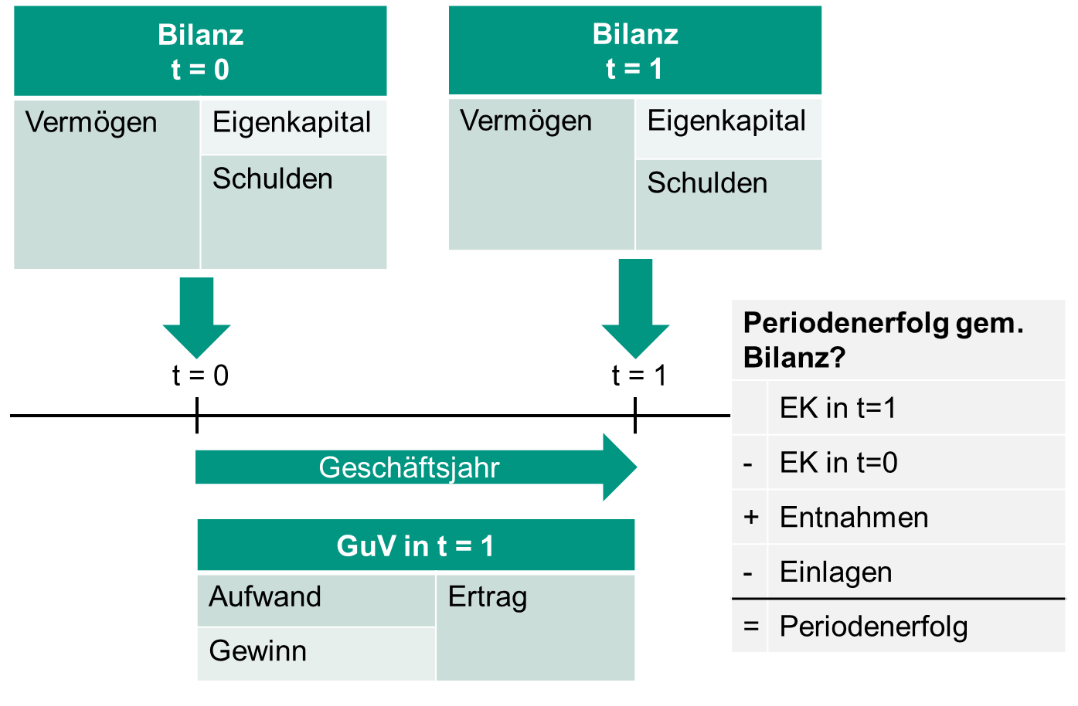
\includegraphics[width=0.7\textwidth]{images/guv.png}
\end{center}
\begin{itemize}
	\item Pflicht zur Aufstellung einer GuV in \textbf{Konto-} oder \textbf{Staffelform}
	\item \textbf{Jahresüberschuss}, wenn Erträge $\geq$ Aufwendungen, \textbf{Jahresfehlbetrag}, wenn Erträge $<$ Aufwendungen
\end{itemize}

\textbf{Gliederung der GuV}:
\begin{itemize}
	\item Keine Vorschriften für \textbf{Personengesellschaften}
	\item Für \textbf{Kapitalgesellschaften} und \textbf{bestimmten Personengesellschaften} ist die GuV in Staffelform darzustellen. Zwei mögliche Verfahren: \textbf{Gesamtkostenverfahren} oder \textbf{Umsatzkostenverfahren}
\end{itemize}
\begin{center}
	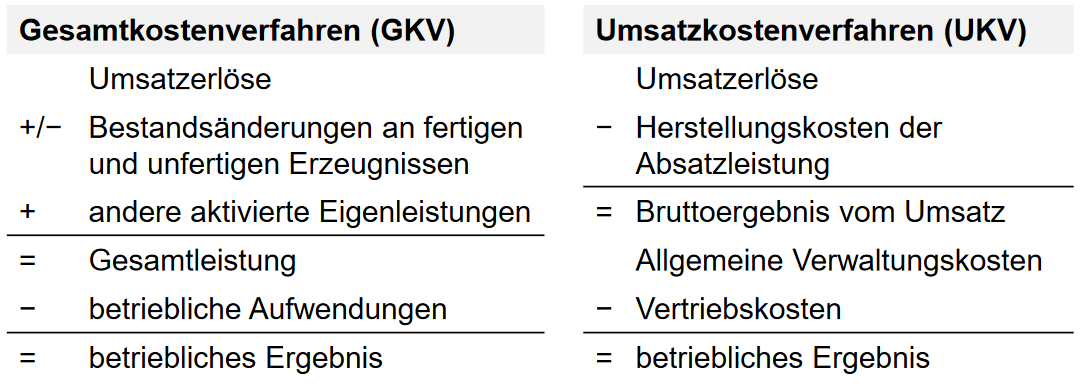
\includegraphics[width=0.7\textwidth]{images/gkvukv.png}
\end{center}
\begin{itemize}
	\item \textbf{Mindestgliederungsvorschriften} nach Größe der KapG (s. FS6/13-16 und 21-29 \textbf{ANSCHAUEN})
	\item \textbf{Pro GKV}: Einfache Integration in Finanzbuchführung,  Gesamtleistung errechenbar,
	Wesentliche Aufwandsarten werden ausgeschrieben,  Keine Kostenstellenrechnung erforderlich
	\item \textbf{Contra GKV}: Körperliche Inventuren, Inkongruenz zwischen Kosten und Leistungsgrößen
	\item \textbf{Pro UKV}: Aussagefähigeres Betriebsergebnis, Zusammenhang zwischen Kosten und Leistungen sichtbar, Körperliche Inventuren entfallen, Internationale Vergleichbarkeit von GuV-Rechnungen
	\item \textbf{Contra UKV}: Kostenstellenrechnung notwendig, Beiträge zur Fixkostendeckung nicht ermittelbar
	\item Abweichungen wie S. 35 Grundsätze für die Gliederung der Bilanz letzten 3 
	\item Kleine und mittlere KapG müssen bei der GuV nur das \textbf{Rohergebnis} ausweisen
	\begin{center}
		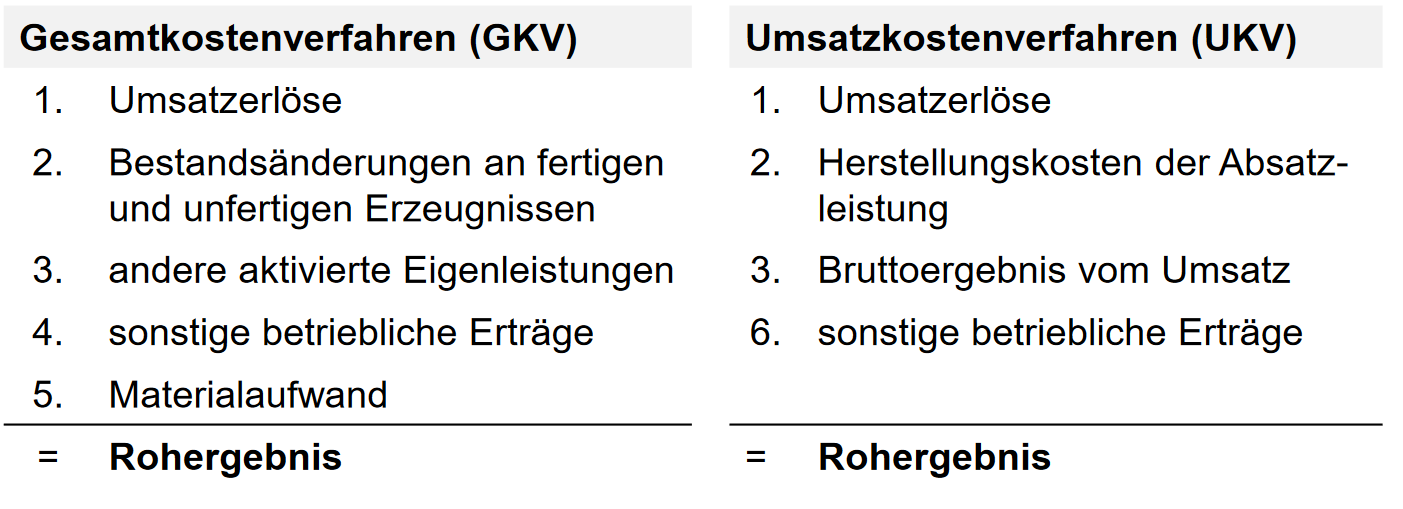
\includegraphics[width=0.7\textwidth]{images/roh.png}
	\end{center}
\end{itemize}

\textbf{Ausweisvorschriften für einzelne Posten der GuV}:
\begin{itemize}
	\item \textbf{Umsatzerlöse}: Ausweisen von allen Erlösen, Erlösschmälerungen und Umsatzsteuer können abgezogen werden
	\item \textbf{Bestandsveränderungen}: Berücksichtigung von Mengen- und Wertänderungen sowie Abschreibungen
	\item \textbf{Außerplanmäßige Abschreibungen}: Gesonderter Ausweis oder Angabe im Anhang
	\item \textbf{Sonstige Erträge und Aufwendungen}: Aus der Abzinsung oder Währungsumrechnung
\end{itemize}
\bigskip
\textbf{Ergebnisverwendungsrechnung}: Soll aufzeigen, aus welchen Mitteln die Ausschüttungen an Aktionäre erfolgen. AktG gibt eine Mustergliederung für die Ergebnisverwendungsrechnung vor (FS6/38+42).

\textbf{AUFGABEN RECHNEN}!!!!



